\documentclass[a4paper, 14pt]{article}
\usepackage[T2A]{fontenc}
\usepackage[utf8]{inputenc}
\usepackage[english,russian]{babel} 

\title{Простые эвристические методы частичного обучения: self-training, co-training, co-learning.}
\author{Николаев Андрей}
%\date{22 ноября 2020}

\usepackage{natbib}
\usepackage{graphicx}
\usepackage{amsmath}
\usepackage{xcolor}

\usepackage{booktabs}

\renewcommand{\familydefault}{\sfdefault}

\usepackage{mathtools}
\usepackage{amsfonts}

\renewcommand{\sinh}{\text{sh}}
\renewcommand{\cosh}{\text{ch}}
\renewcommand{\tanh}{\text{th}}
\renewcommand{\tan}{\text{tg}}
\renewcommand{\arctan}{\text{arctg}}

\newcommand{\bounds}{\left[2;3\right]}
\newcommand{\upperbound}{3}
\newcommand{\lowerbound}{2}

\newcommand{\myoperator}{(Af)(x) = -(x^2+4)f''(x)-2xf'(x)}
\newcommand{\myarea}{\left \{ f \in W^{2,2}\left(\bounds\right): \quad f\left(\lowerbound\right) = \pi f'\left(\lowerbound\right), \quad f'(\upperbound) = 0 \right \}}

\title{Простые эвристические методы частичного обучения: self-training, co-training, co-learning.}
\author{Николаев Андрей}
%\date{Вариант 7}

\begin{document}
\maketitle
\section{Частичное обучение}
\subsection{Постановка задачи}
Существует привычная нам задача классификации. Мы имеем $X$ --- множество объектов с известными признаками и $Y$ --- пространство классов. Есть неизвестная функция $X \longrightarrow Y$, сопоставляющая каждому обьекту его класс. Имеется обучающая выборка $\{x_1, x_2, ...\} \subset X$ и соответствующие им известные классы $\{y_1, y_2, ...\} \subset Y$. Задача классификации сводится к построению классификатора --- некой аппроксимации неизвестной функции $X \longrightarrow Y$. \\

С другой стороны существует задача кластеризации. Мы все также имеем $X$ --- множество объектов. И хотим аппроксимировать функцию $X \longrightarrow Y$. Но на этот раз у нас нет обучающей выборки, зато есть функция расстояния между объектами $\rho: X\times X \longrightarrow \mathbb{R}$. И в этом случае кластеризующая функция строится не на основе обучающей выборки, а так чтобы расстояние между объектами одного кластера было мало, а расстояние между объектами разных кластеров было велико. \\

Первый случай называется обучение с учителем,а кластеризация называется обучением без учителя. Где-то по середине между этими задачами находится задача частичного обучения. В этом случае у нас все также есть множество обьектов из $X$ и (возможно) функция $\rho$. При этом только для некоторой доли имеющихся обьектов известна классовая принадлежность. Иначе говоря обучающая выборка размечена \textbf{частично}. \\

Приведем пример (Рис. 1). Допустим известные обьекты в пространстве признаков имеют вид в виде двух бананов. И нам известна принадлежность только двух точек. В таком случае чистая задача кластеризации обучит классификатор только по двум точкам, который будет иметь сомнительное качество на всех остальных данных. При это частичное обучение могло бы учесть явную кластеризацию данных и дать значительно лучшую классификацию.\\

\begin{center}
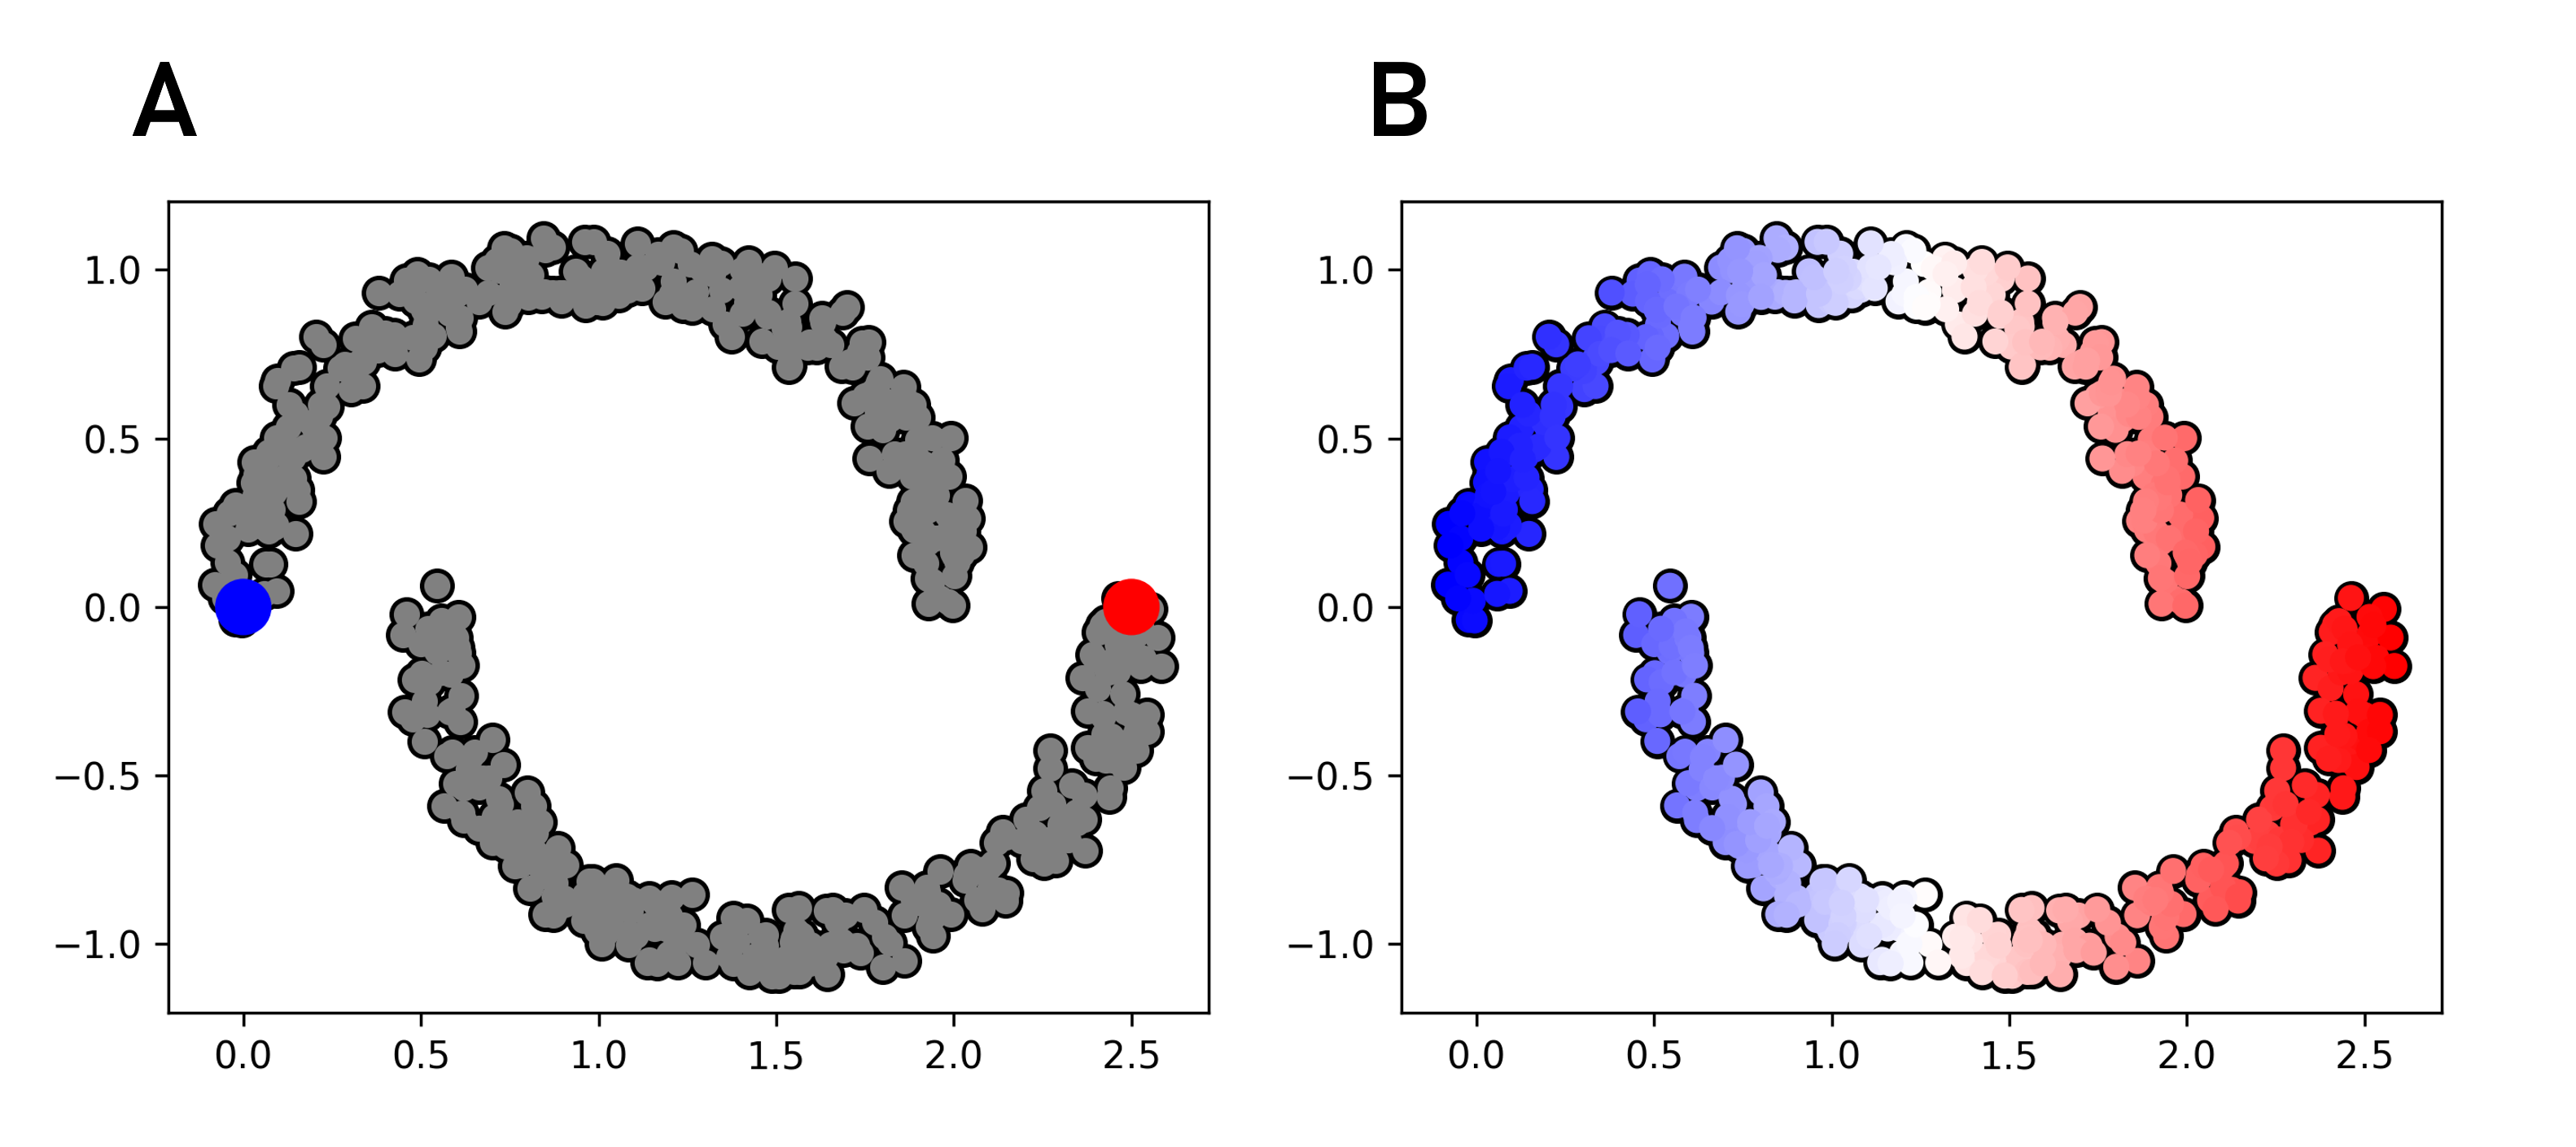
\includegraphics[width=1.0\textwidth]{picture_1.png}
\textbf{Рисунок 1.} (\textbf{A}) Пример частично размеченных данных. (\textbf{B}) Классификация обученная на размеченных данных не учитывает кластерную структуру неразмеченных. 
\end{center}

Однако частичное обучение не может сводиться только к кластеризации, представьте теперь, что мы знаем классы уже трех точек на выборке из двух бананов (Рис. 2). В таком случае кластеризация дала бы предсказание которое не может соотноситься с известными классами всех трех точек. Таким образом задача частичного обучения действительно находится посередине между классификацией и кластеризацией, но не является ни тем, ни другим. \\
\begin{center}
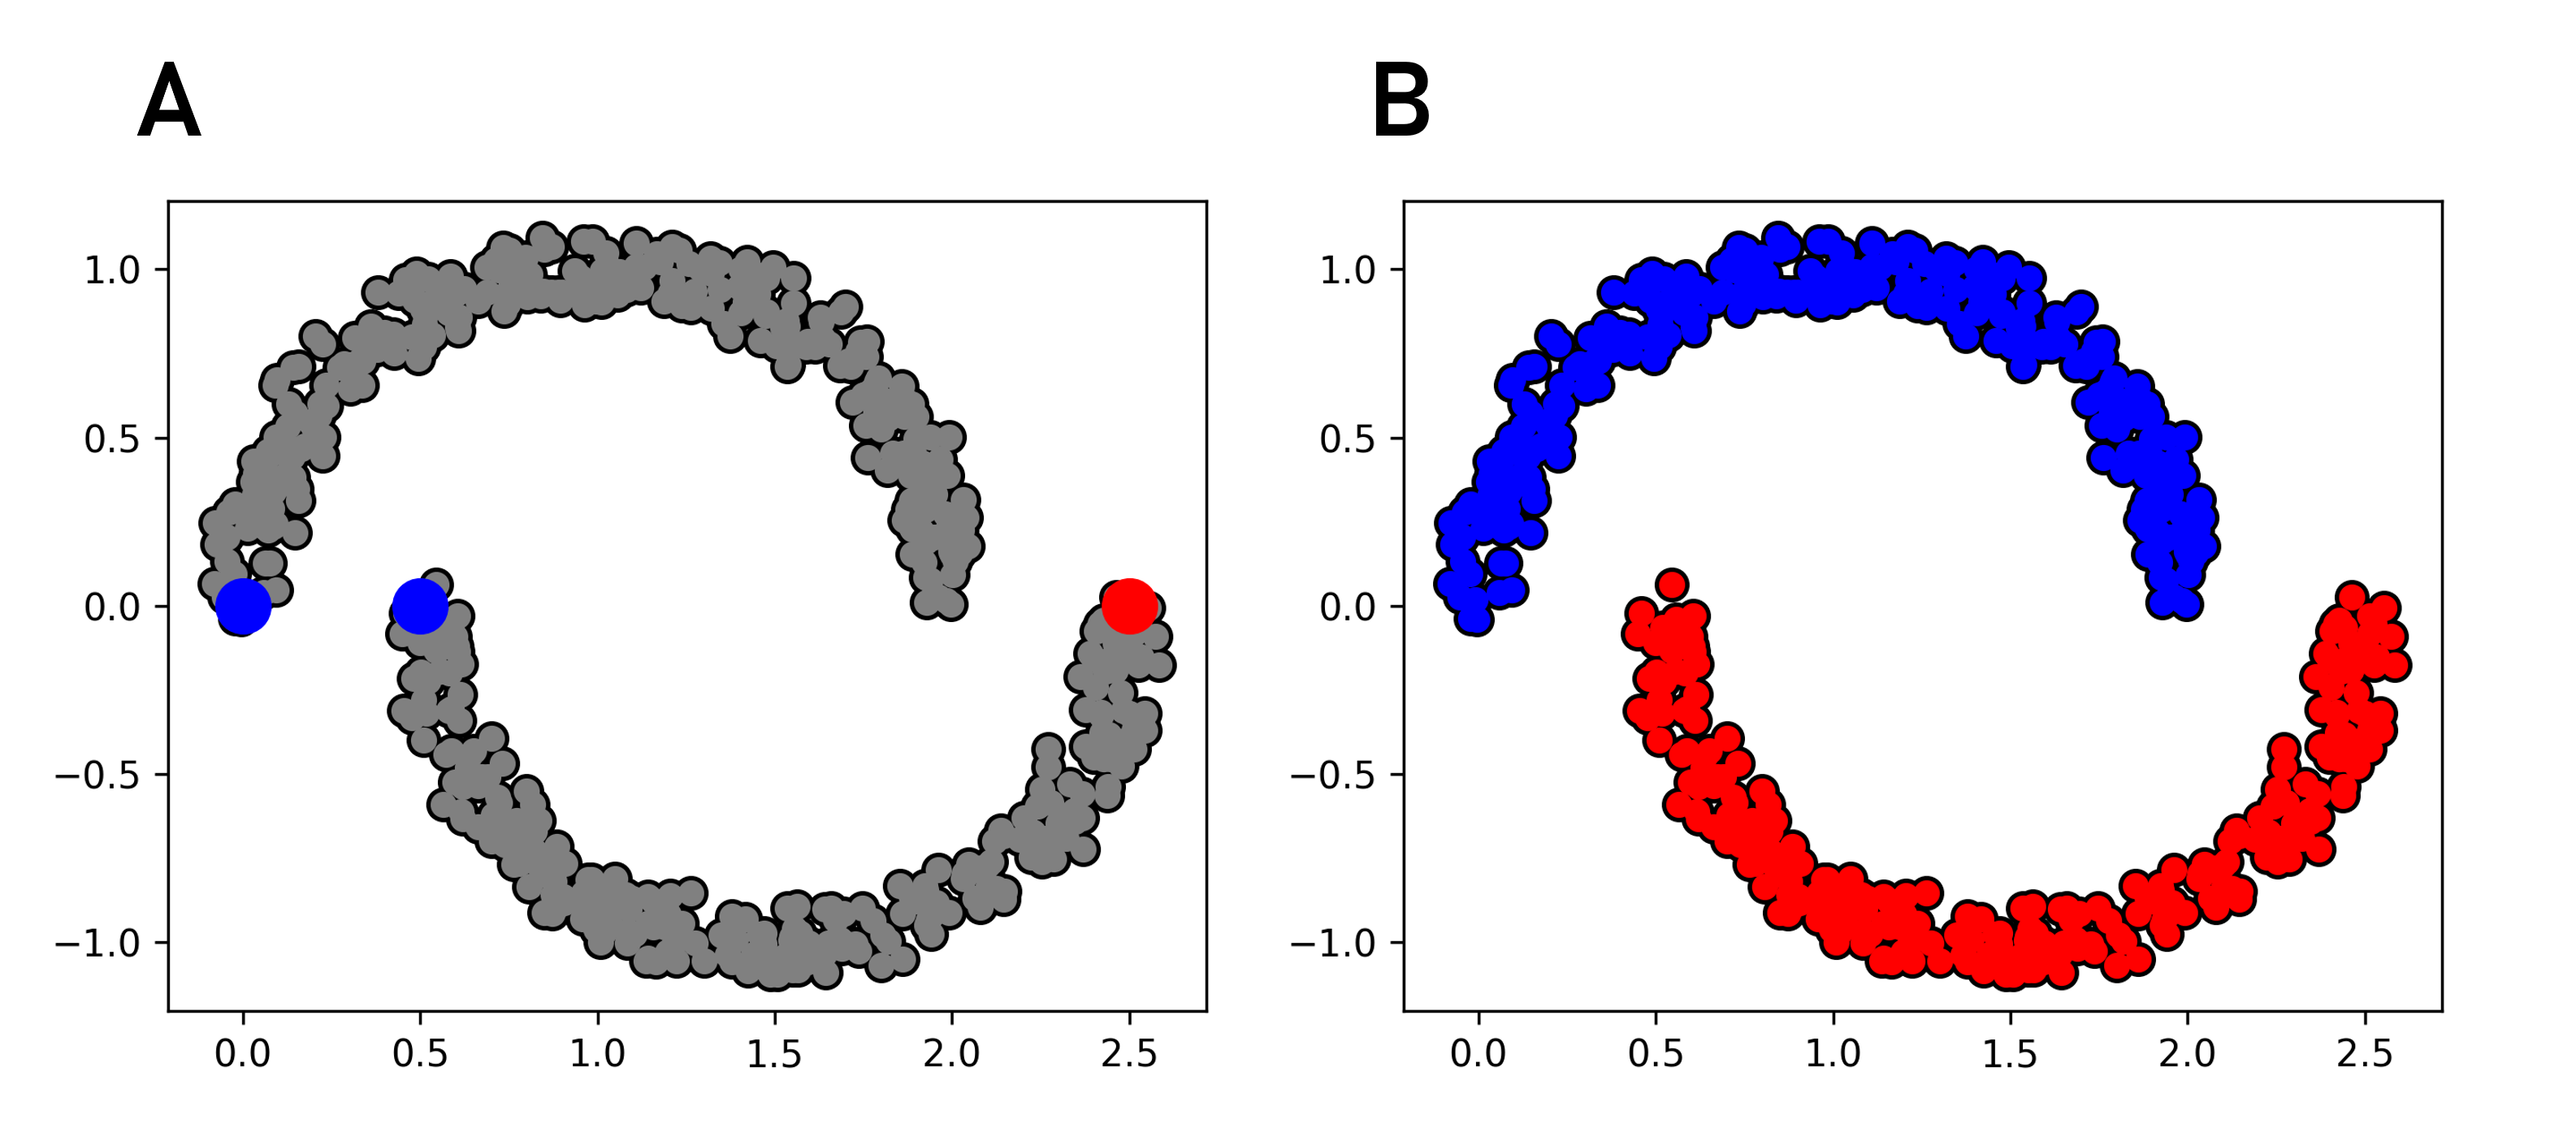
\includegraphics[width=1.0\textwidth]{picture_2.png}
\textbf{Рисунок 2.} (\textbf{A}) Пример частично размеченных данных. (\textbf{B}) Кластеризация не учитывает классовую принадлежность размеченных данных. 
\end{center}

Приведем пример: программист решил сделать классификатор для фотографий котиков и собачек, для этого он скачал по миллиону фотографий и тех и других. Однако, ему хватило сил подписать котик это или собачка только для 1000 фотографий. Классификация не может быть построена только по 1000 фотографиям --- мало данных, а кластеризация может разбить фотографии неизвестным образом --- по цвету фона, по размеру животного. И только частичное обучение может помочь ленивому программисту.
\subsection{Self-training}
Каким же образом можно реализовать частичное обучение? Рассмотрим подход, который называется self-training (само-обучение). Вернемся к датасету с бананами в котором известны классы двух точек. Как было сказано ранее построение классификатора по двум точкам тут не поможет. Однако допустим, что мы все же построили классификатор по двум точкам, к примеру логистическую регрессию. Вспомним что многие методы классификации могут оценивать свою уверенность в предсказании. Тогда для некоторых точек с наибольшей уверенностью классификации (скажем 5\% самых уверенных) предсказание  классификации может оказаться вполне верным. Давайте же дополним обучающую выборку классификатора этими точками. На второй итерации нашего подхода мы обучим классификатор уже по дополненной обучающей выборке. Выполнив предсказание для остальных данных, выберем еще раз 5\% ранее неразмеченных точек с наибольшей уверенностью и пополним ими обучающую выборку. Будем повторять такие итерации пока не классифицируем все точки в нашем датасета. Как мы видим, результат такого подхода заметно лучше, чем у классификации по двум исходным точкам. 
\begin{center}
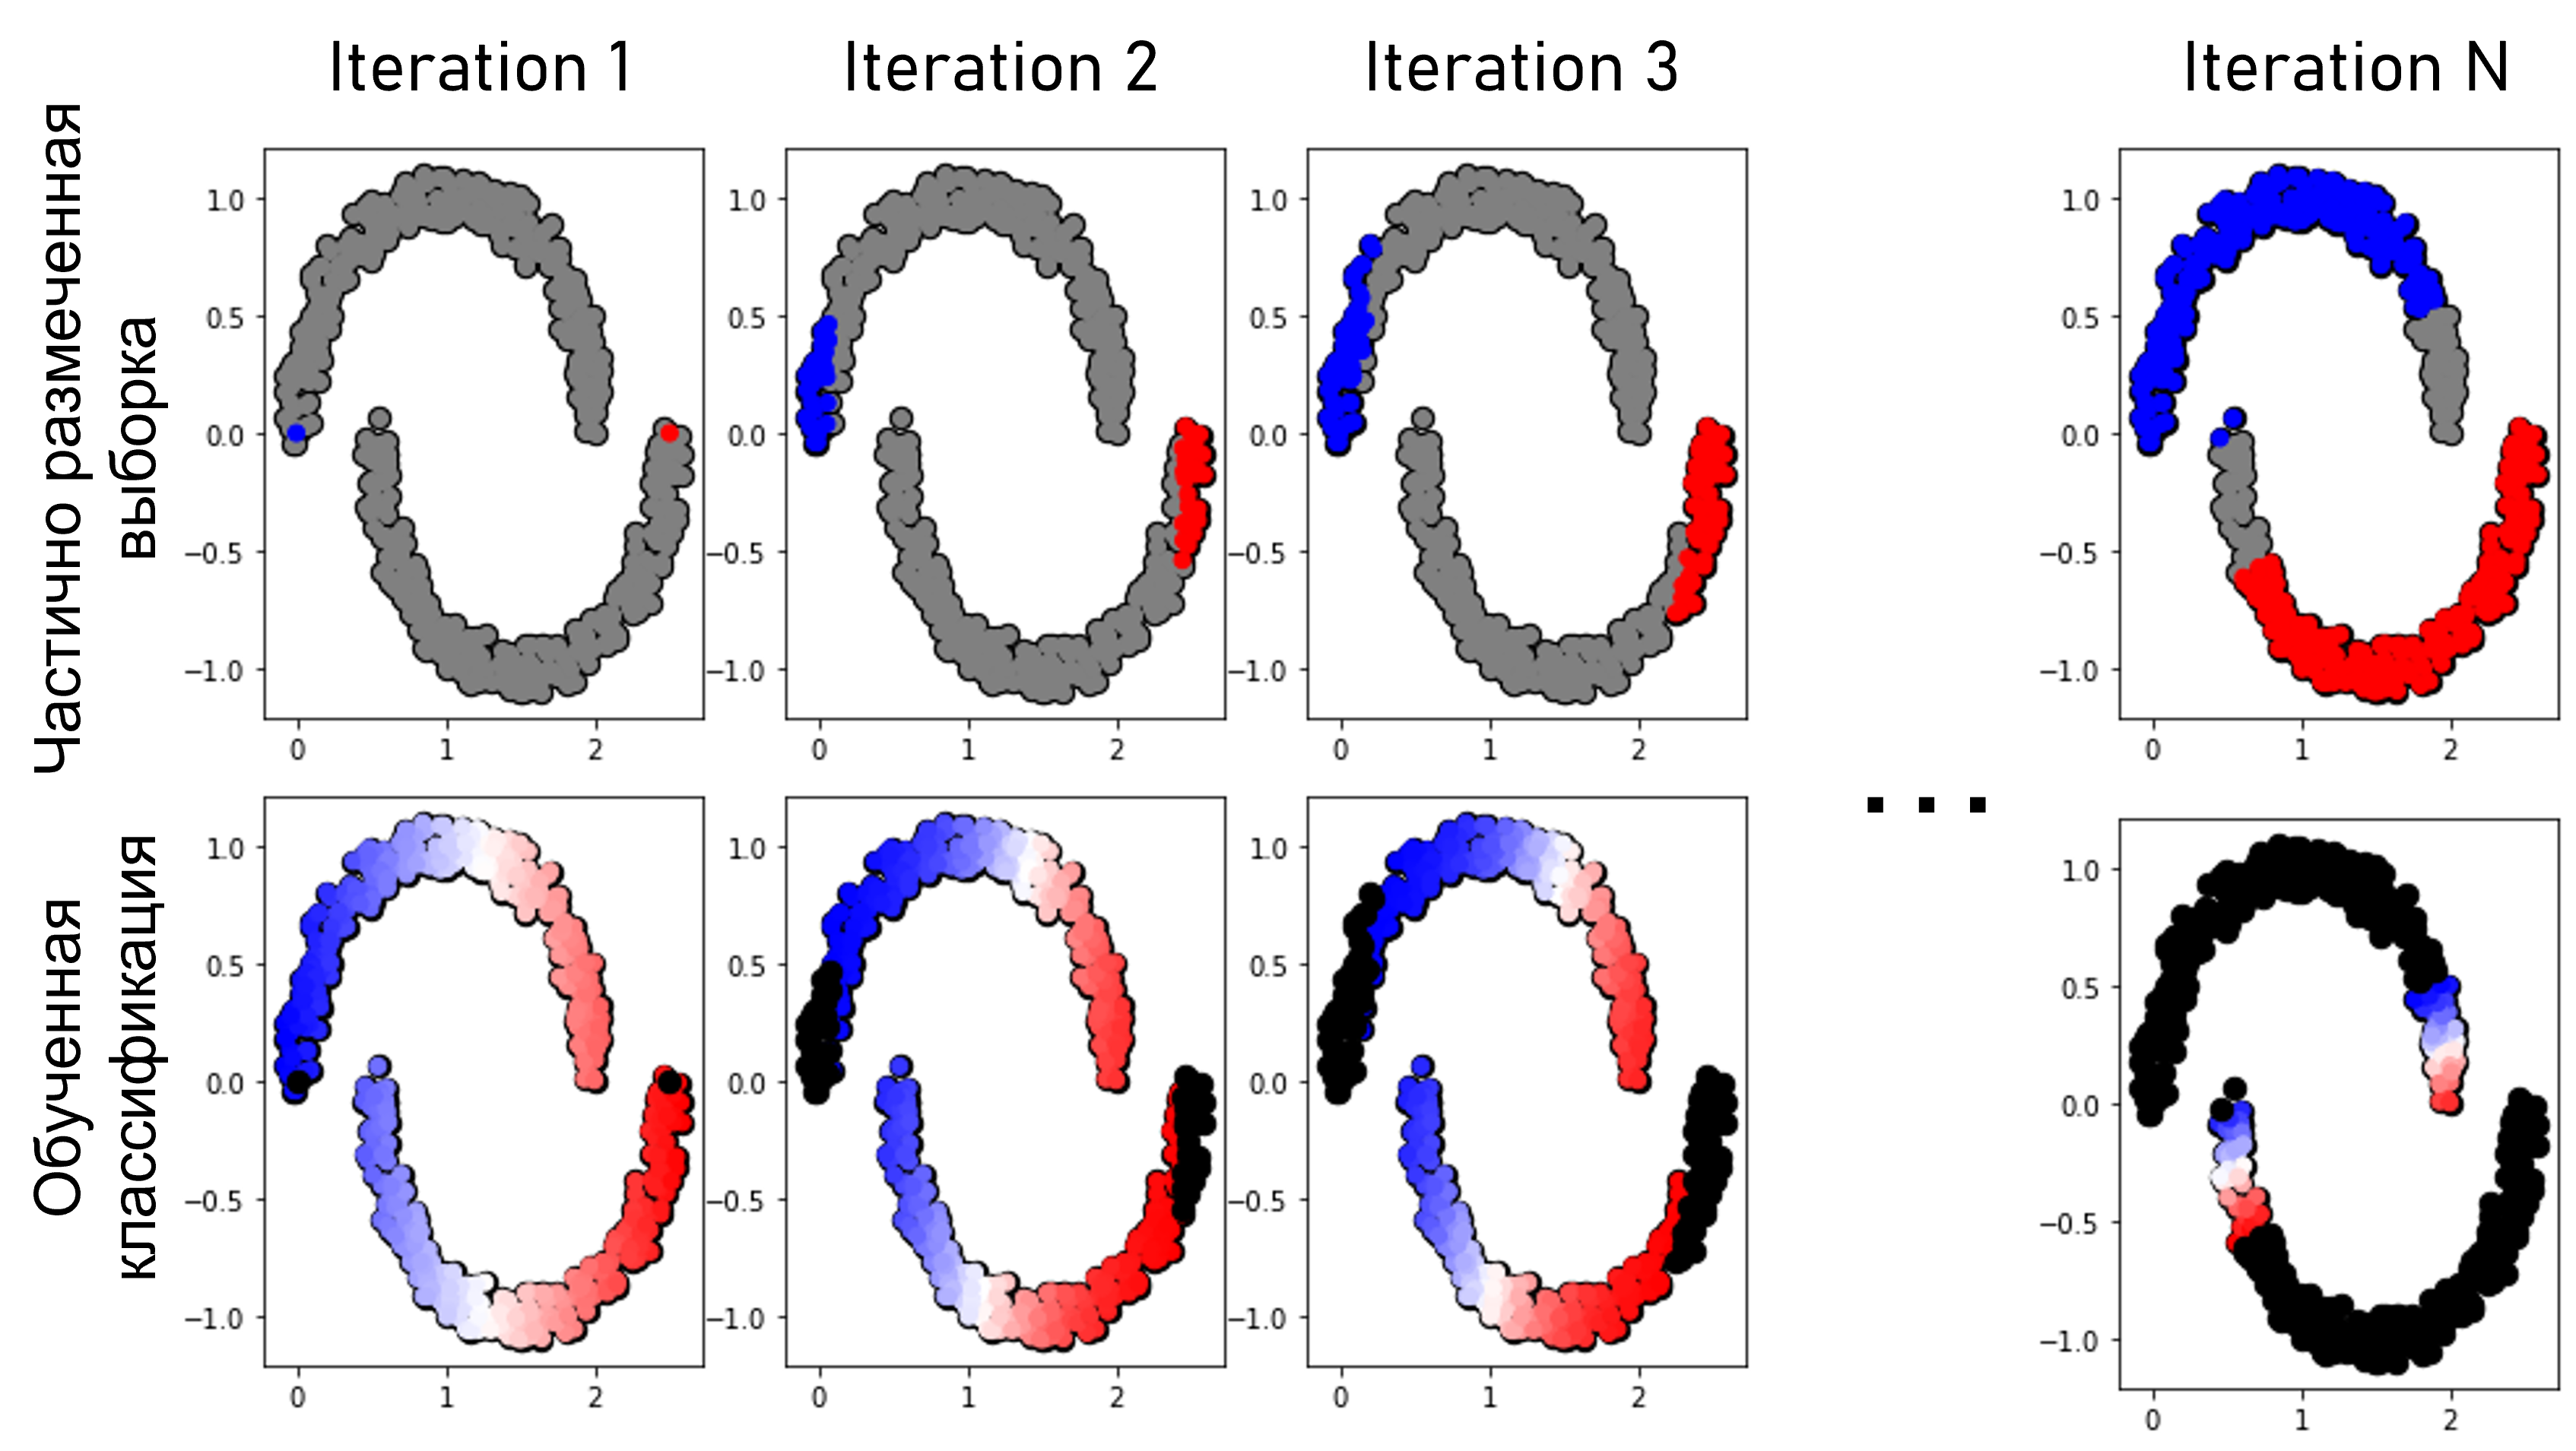
\includegraphics[width=1.0\textwidth]{picture_3.png}
\textbf{Рисунок 3.} Пример работы итераций self-training. 
\end{center}
Оформим описанный процесс более математизировано. Пусть мы строим функцию $a: X \longrightarrow Y$. Пусть у нас есть метод обучения функции $\mu: Z \longrightarrow a$ который принимает на вход размеченную часть выборки $Z \subset X$. Допустим функция $a$ имеет вид
\begin{equation*}
    a(x) = \arg \max_{y \subset Y}\Gamma_y(x)
\end{equation*}
где $\Gamma_y(x)$ это некоторые (к примеру) линейные функции от $x \subset X$ которые обучаются так, чтобы быть большими, если $x$ принадлежит классу $y$ и маленькими в противном случае. В таком случае уверенность классификации в принадлежности элемента $x$ к классу $y_1$ (отступ):
\begin{equation*}
    M_1(x) = \Gamma(x) - \max_{y \subset Y\backslash y_1}\Gamma_{y_1}(x) 
\end{equation*}
Пусть $Z$ это размеченная часть обучающей выборки. Тогда алгоритм выглядит так:
\begin{enumerate}
  \item $a = \mu(Z)$ --- обучить классификатор на размеченной выборке
  \item $\Delta := \{x \subset X\backslash Z \;|\; M(x) \geq M_0 \}$ --- выбрать несколько точек из неразмеченной части выборки которые наиболее уверенно классифицируются. 
  \item $Z := Z\cup\Delta$ --- дополнить размеченную выборку
  \item Если не все элементы выборки размечены, вернуться в начало.
\end{enumerate}
\subsection{Сo-training}
Рассмотрим более узкий кейс, допустим у нас есть не один, а целых два метода обучения классификации $\mu_1, \mu_2$, которые принципиально отличаются друг от друга, например имеют разные парадигмы обучения, и/или используют разные признаки обьектов, и/или имеют разную стартовую выборку. В таком случае мы можем получить преимущество в частичном обучении заставив их учить друг друга по следующему алгоритму:
\begin{enumerate}
  \item $a_1 = \mu_1(Z_1)$\\
  $a_2 = \mu_2(Z_2)$ --- два метода обучают классификаторы на своих размеченных выборках. 
  \item $\Delta_1 := \{x \subset X\backslash Z_1\backslash Z_2 \;|\; M_1(x) \geq M_{01} \}$ --- метод 1 размечает неразмеченные точки, в которых он уверен.\\
  $\Delta_2 := \{x \subset X\backslash Z_1\backslash Z_2 \;|\; M_2(x) \geq M_{02} \}$ --- метод 2 делает тоже самое.
  \item $Z_1 := Z_1\cup\Delta_2$ --- метод 2 дополняет обучающую выборку метода 1 \\
  $Z_2 := Z_2\cup\Delta_1$ --- метод 1 дополняет обучающую выборку метода 2
  \item Если не все элементы выборки размечены, вернуться в начало.
\end{enumerate}
\subsection{Сo-learning}
Идем еще дальше, допустим у нас теперь есть набор методов $\mu_i$ отличающиеся чем-то. Допустим что все эти методы обучились на одной выборке $Z$ и произвели классификаторы $a_i$. Давайте соберем из множества классификаторов $a_i$ один классификатор-мегазорд:
\begin{equation*}
    a(x) = \arg \max_{y \subset Y}\Gamma_y(x)
\end{equation*}
Где на этот раз функции $\Gamma$ определяются как:
\begin{equation*}
    \Gamma_y(x) = \sum_{i = 1}^{I}[a_i(x) = y]
\end{equation*}
Выражение в квадратных скобках равно 1 когда написанное в них верно, и равно 0 в противных случаях. Иначе говоря, классификаторы $a_i$ голосуют за принадлежность к классам, и демократически выбирают к кому классу отнести каждый из обьектов. Далее на основе такого обьединенного классификатора строится Self-training описанный выше. 
\subsection{Задачи}
\subsection*{Задача 1}
Возможно ли при помощи self-training эффективно классифицировать точки частично размеченной выборки представленной ниже:
\begin{center}
\includegraphics[width=0.5\textwidth]{picture_5.png}
\end{center}
\textit{\textbf{Решение:} Конечно можно! Для этого нужно построить self-training на основе классификатора который может делать разделяющую поверхность в виде окружности, например классификаторы восстанавливающие плотность или логистическая регрессия с добавлением квадратичных признаков}
\subsection*{Задача 2}
Два подхода частичного обучения применяются для классификации обьектов частичной выборки представленной ниже.
\begin{center}
\includegraphics[width=0.5\textwidth]{picture_4.png}
\end{center}
Первый подход это self-training на основе логичтической регрессии, которая видит только первый признак. Второй подход это co-training на основе двух логистических регрессий, таких что первая видит первый признак, а вторая второй. Какой алгоритм приведет к лучшей классификации точек и почему?\\

\textit{\textbf{Решение:} self-training видящий только первый признак веротянее всего идеально классифицирует точки, так как по этому признаку кластеры разделены и практически не пересекаются. В случае co-training классификатор использующий второй признак видит кластеры пересекающимися и почти наверняка наделает ошибок при классификации}
\subsection*{Задача 3}
Алгоритм co-training построенный на основе трех классификаторов классифицирует точки представленной ниже выборки. На последней итерации работы алгоритма осталась лишь одна неклассифицированная точка. На этот момент классификаторы имеют разделяющие линии представленные на картинке. К какому кластеру будет отнесена оставшаяся точка?
\begin{center}
\includegraphics[width=0.5\textwidth]{picture_6.png}
\end{center}
\textit{\textbf{Решение:} Судя по разделяющим линиям два классификатора проголосую за красный кластер, и только один за синий, в итоге точка будет отнесена к красному кластеру.}


\end{document}
